\chapter{The CMS Experiment}
\label{chapter:experiment}

\section{The Large Hadron Collider}
\label{sec:lhc}

\begin{figure}[!htbp]
    \centering
    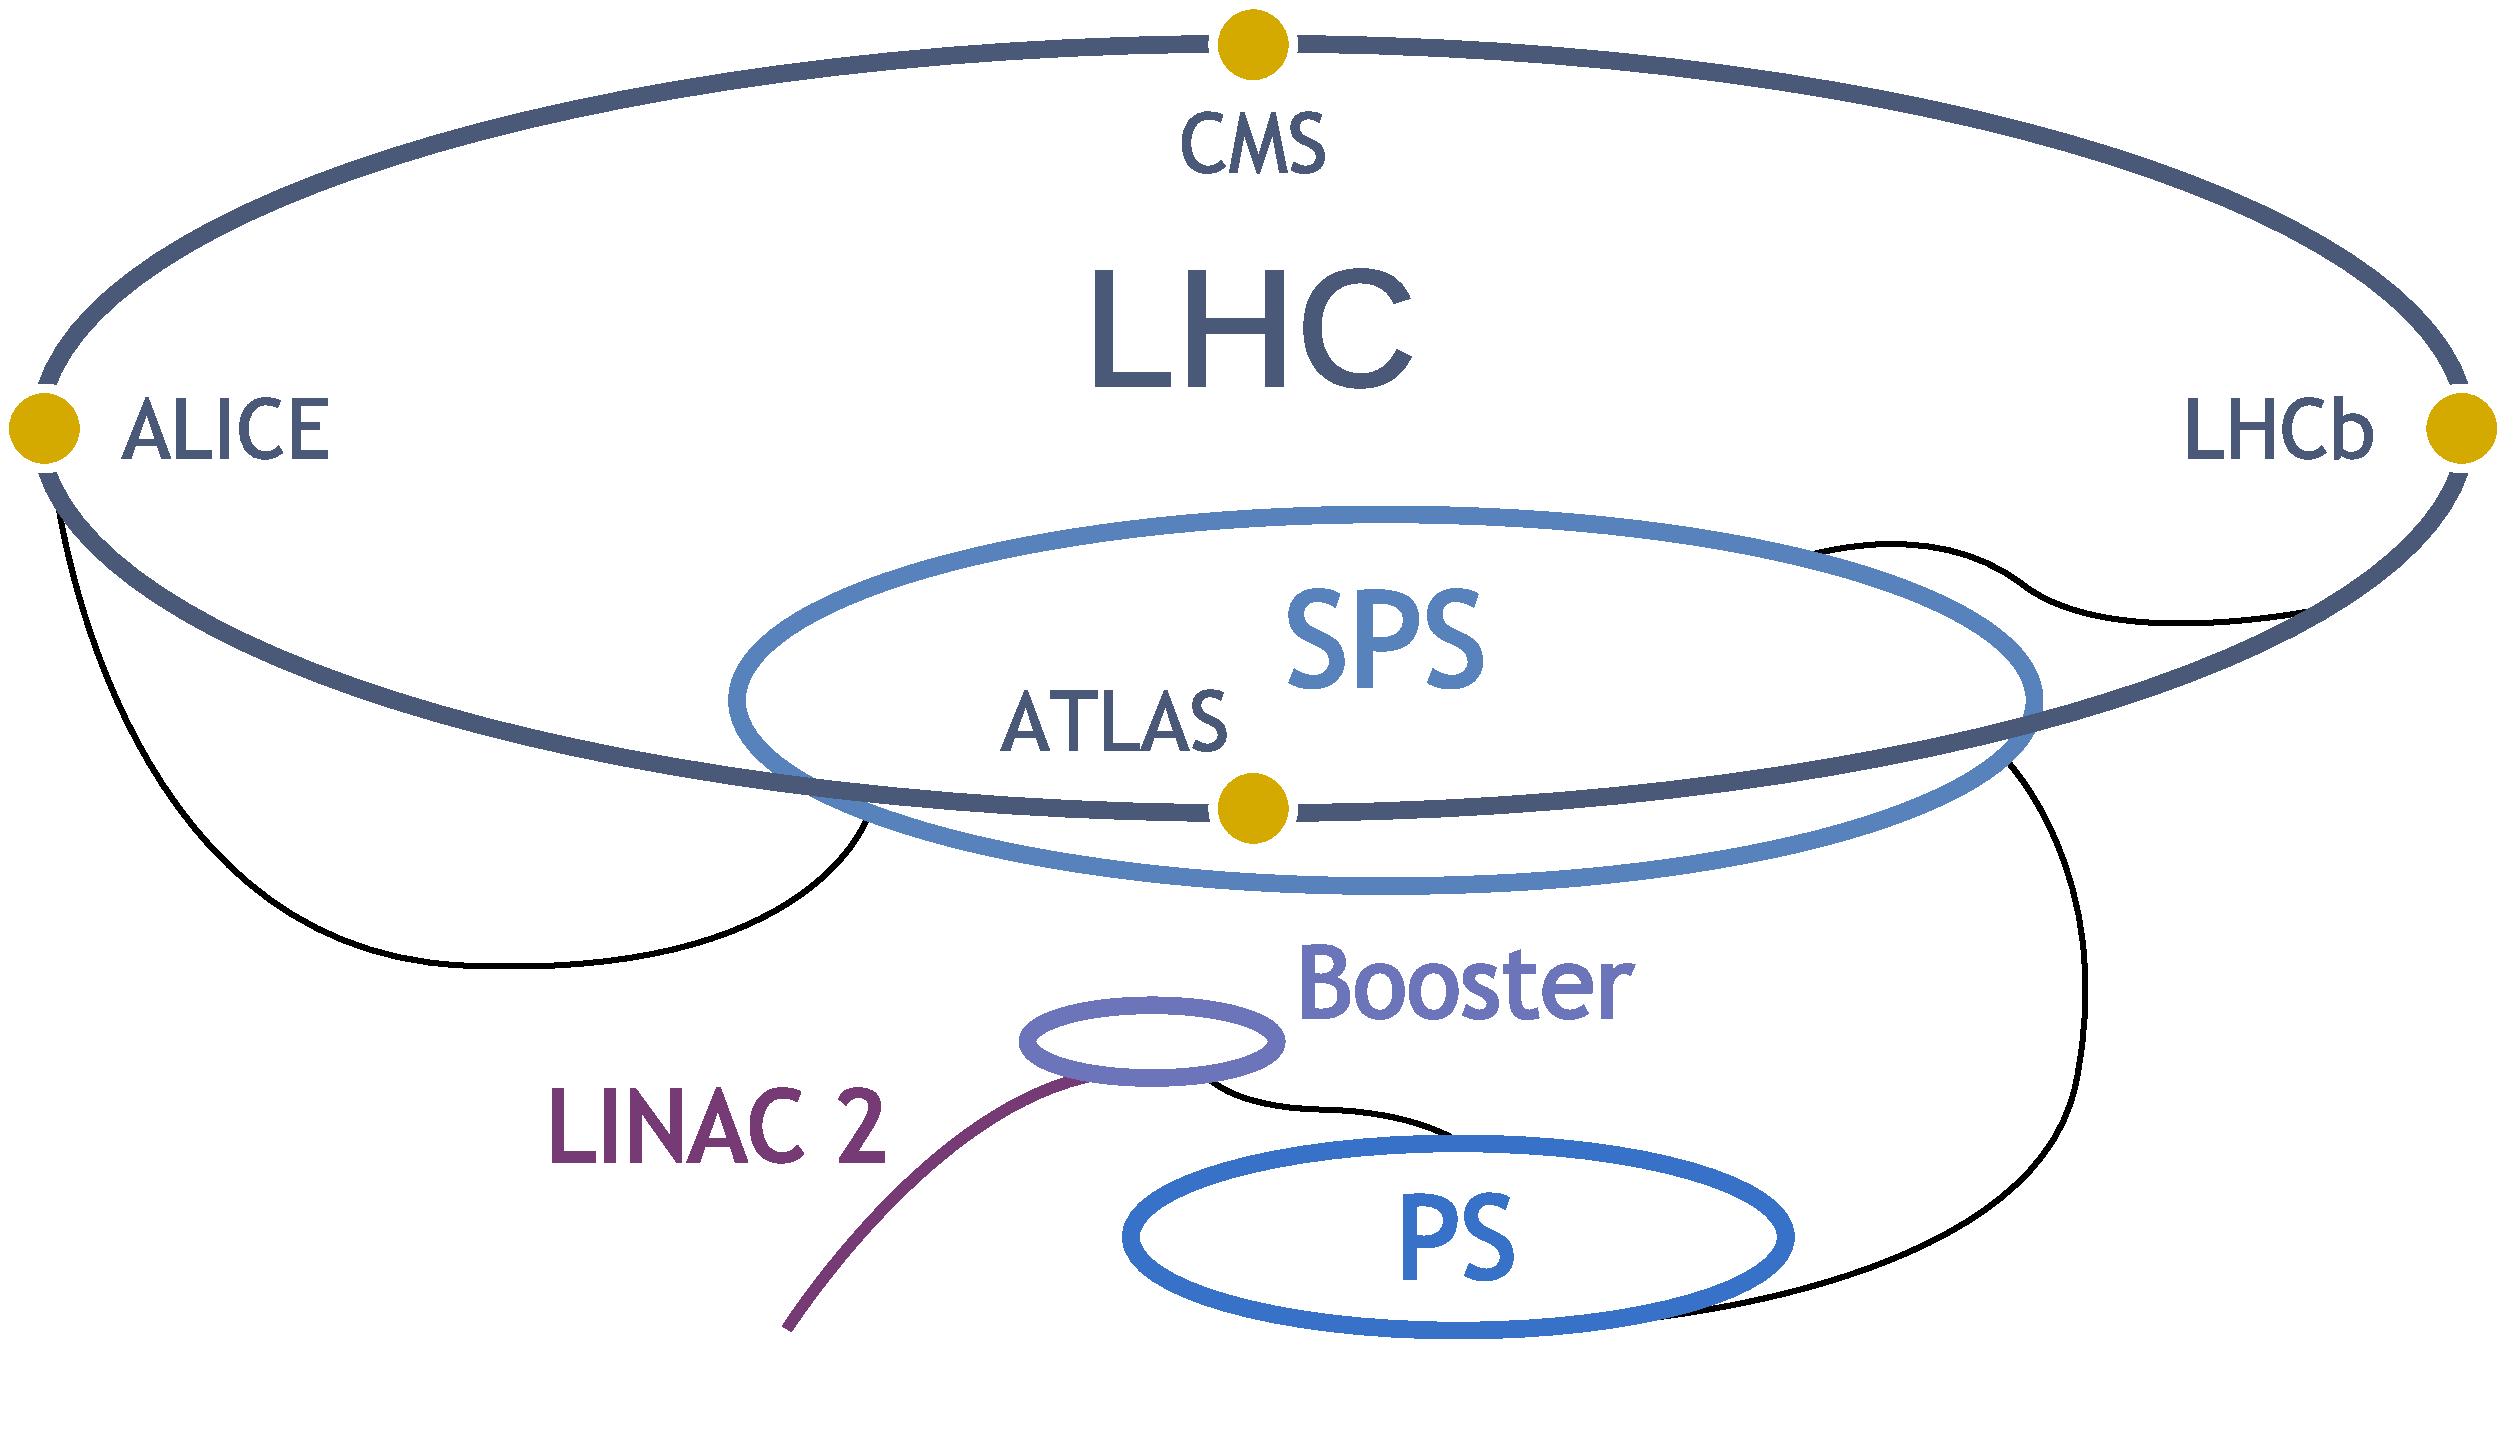
\includegraphics[width=\textwidth]{figures/alex_lhc_layout.pdf}
    \caption[
        A schematic view of the LHC and the location of the four experiments.
    ]{
        A schematic view of the LHC and the location of the four experiments.
        Also shown are the accelerators that feed protons into the LHC.
    }
    \label{fig:lhc_layout}
\end{figure}

The Large Hadron Collider (LHC) is the world's highest energy and largest
particle accelerator with a maximum design center-of-mass energy of 14\TeV and
a radius of 2804\meters \cite{bruning2004}. It collides protons on protons, as
well as protons on ionized lead (\lead) and \lead on \lead. In 2012, when LHC
most recently produced collisions, it had a center of mass energy of 8\TeV;
when it turns back on in 2015 after upgrades, it will run at 13\TeV. The LHC is
located near Geneva, Switzerland, although it is so large that most of the
accelerator (including \pointfive, where the CMS detector is located) is in
France.

A number of smaller accelerators are used together in series to accelerate
protons to the energies necessary to be injected into the LHC. The first step
is a linear accelerator, \linactwo, which accelerates protons from rest to
50\MeV. These protons are then injected into a chain of three circular
accelerators, each injecting into the next. The first of these accelerators is
the Proton Synchrotron Booster (PSB) which accelerates the protons to 1.4\GeV.
The second is the Proton Synchrotron (PS) which accelerates the protons to
26\GeV. The third and final accelerator is the Super Proton Synchrotron (SPS)
which accelerates the protons to 450\GeV and injects directly into the LHC.

Bunches of protons are accelerated using this system and injected into the LHC
to form two counter-rotating beams. When the desired number of bunches have
been injected into the LHC, the LHC accelerates them to 4\TeV. When the beams
have reached their nominal energy, they are focused and brought into collision
at four different points on the ring where the various experiments (\ALICE,
\ATLAS, \LHCB, and CMS) are located. A cartoon layout of the LHC and its
accelerator chain is shown in \FIG~\ref{fig:lhc_layout}.

The beams are steered around the accelerator ring by a series of
superconducting, dipole magnets. When running at a center-of-mass energy of
8\TeV, these magnets operate at roughly 7.5\Tesla. There are also quadrapoles
to focus the beam and some higher order magnets around the ring to correct for
lattice defects. The bunches of protons are accelerated by 16 superconducting
radio frequency cavities. These cavities accelerate slower protons while
slowing faster ones, thereby keeping the proton bunches compact in both real
and momentum space. There is room for 2808 bunches in LHC separated by 25\ns,
although in 2012 50\ns spacing was used and so there were only 1374 bunches of
which 1368 were brought into collision at CMS and \ATLAS.

The LHC is also the highest luminosity collider in the world. The instantaneous
luminosity is given by
\begin{equation}
    \luminosity = f n \frac{N^{2}}{\sigma}
\end{equation}
where $f$ is the frequency of interaction (which is fixed by the LHC's
circumference), $n$ is the number of bunches in a beam, $N$ is the number of
protons per bunch (with the $N^{2}$ coming from the assumption that there are
the same number of protons in the two colliding bunches), and $\sigma$ is the
area profile of the beams.

Although a higher luminosity means more particles are produced and more data
can be collected, the maximum luminosity is limited by several practical
factors. The first factor is cost; a higher luminosity general requires a more
expensive machine as the ring is either made larger or the technology needed to
run the machine is made more complex. The cost of the detectors also increases
as they require more channels to separate the larger number of particles,
faster readout to deal with the increased event rate, and higher bandwidth to
read out the larger numbers of channels. The second is the challenge that
higher luminosities present to the analyzers. The luminosity can be increased
by increasing the number of protons in a bunch or by squeezing the bunches more
tightly, but eventually the probability of getting multiple proton-proton
interactions per bunch crossing becomes large, leading to a phenomenon known as
pileup. These extra interactions add additional particles to the detector and
can make it difficult to separate interesting events from uninteresting
background. The luminosity can also be increased by increasing the number of
bunches in the machine, but this decreases the time between the collisions and
leads to a phenomenon known as out-of-time pileup which can also obscure
interesting events. The third factor is that high radiation doses damage the
detectors. Plastic and crystal scintillators darken while silicon detectors
become noisy. This forces the detectors to replace their components more
frequently.

In 2012, the optimal luminosity was achieved by running with bunches spaced by
50\ns instead of the design nominal bunch spacing of 25\ns. This larger bunch
spacing was chosen because at smaller spacing the bunches were destabilized by
electron clouds---clouds of electrons knocked out of the beam pipe by the
beam's synchrotron radiation, as well as secondary electrons freed when the
photoelectrons impact their surroundings.

\section{The Compact Muon Solenoid}
\label{sec:cms}

\begin{figure}[!htbp]
    \centering
    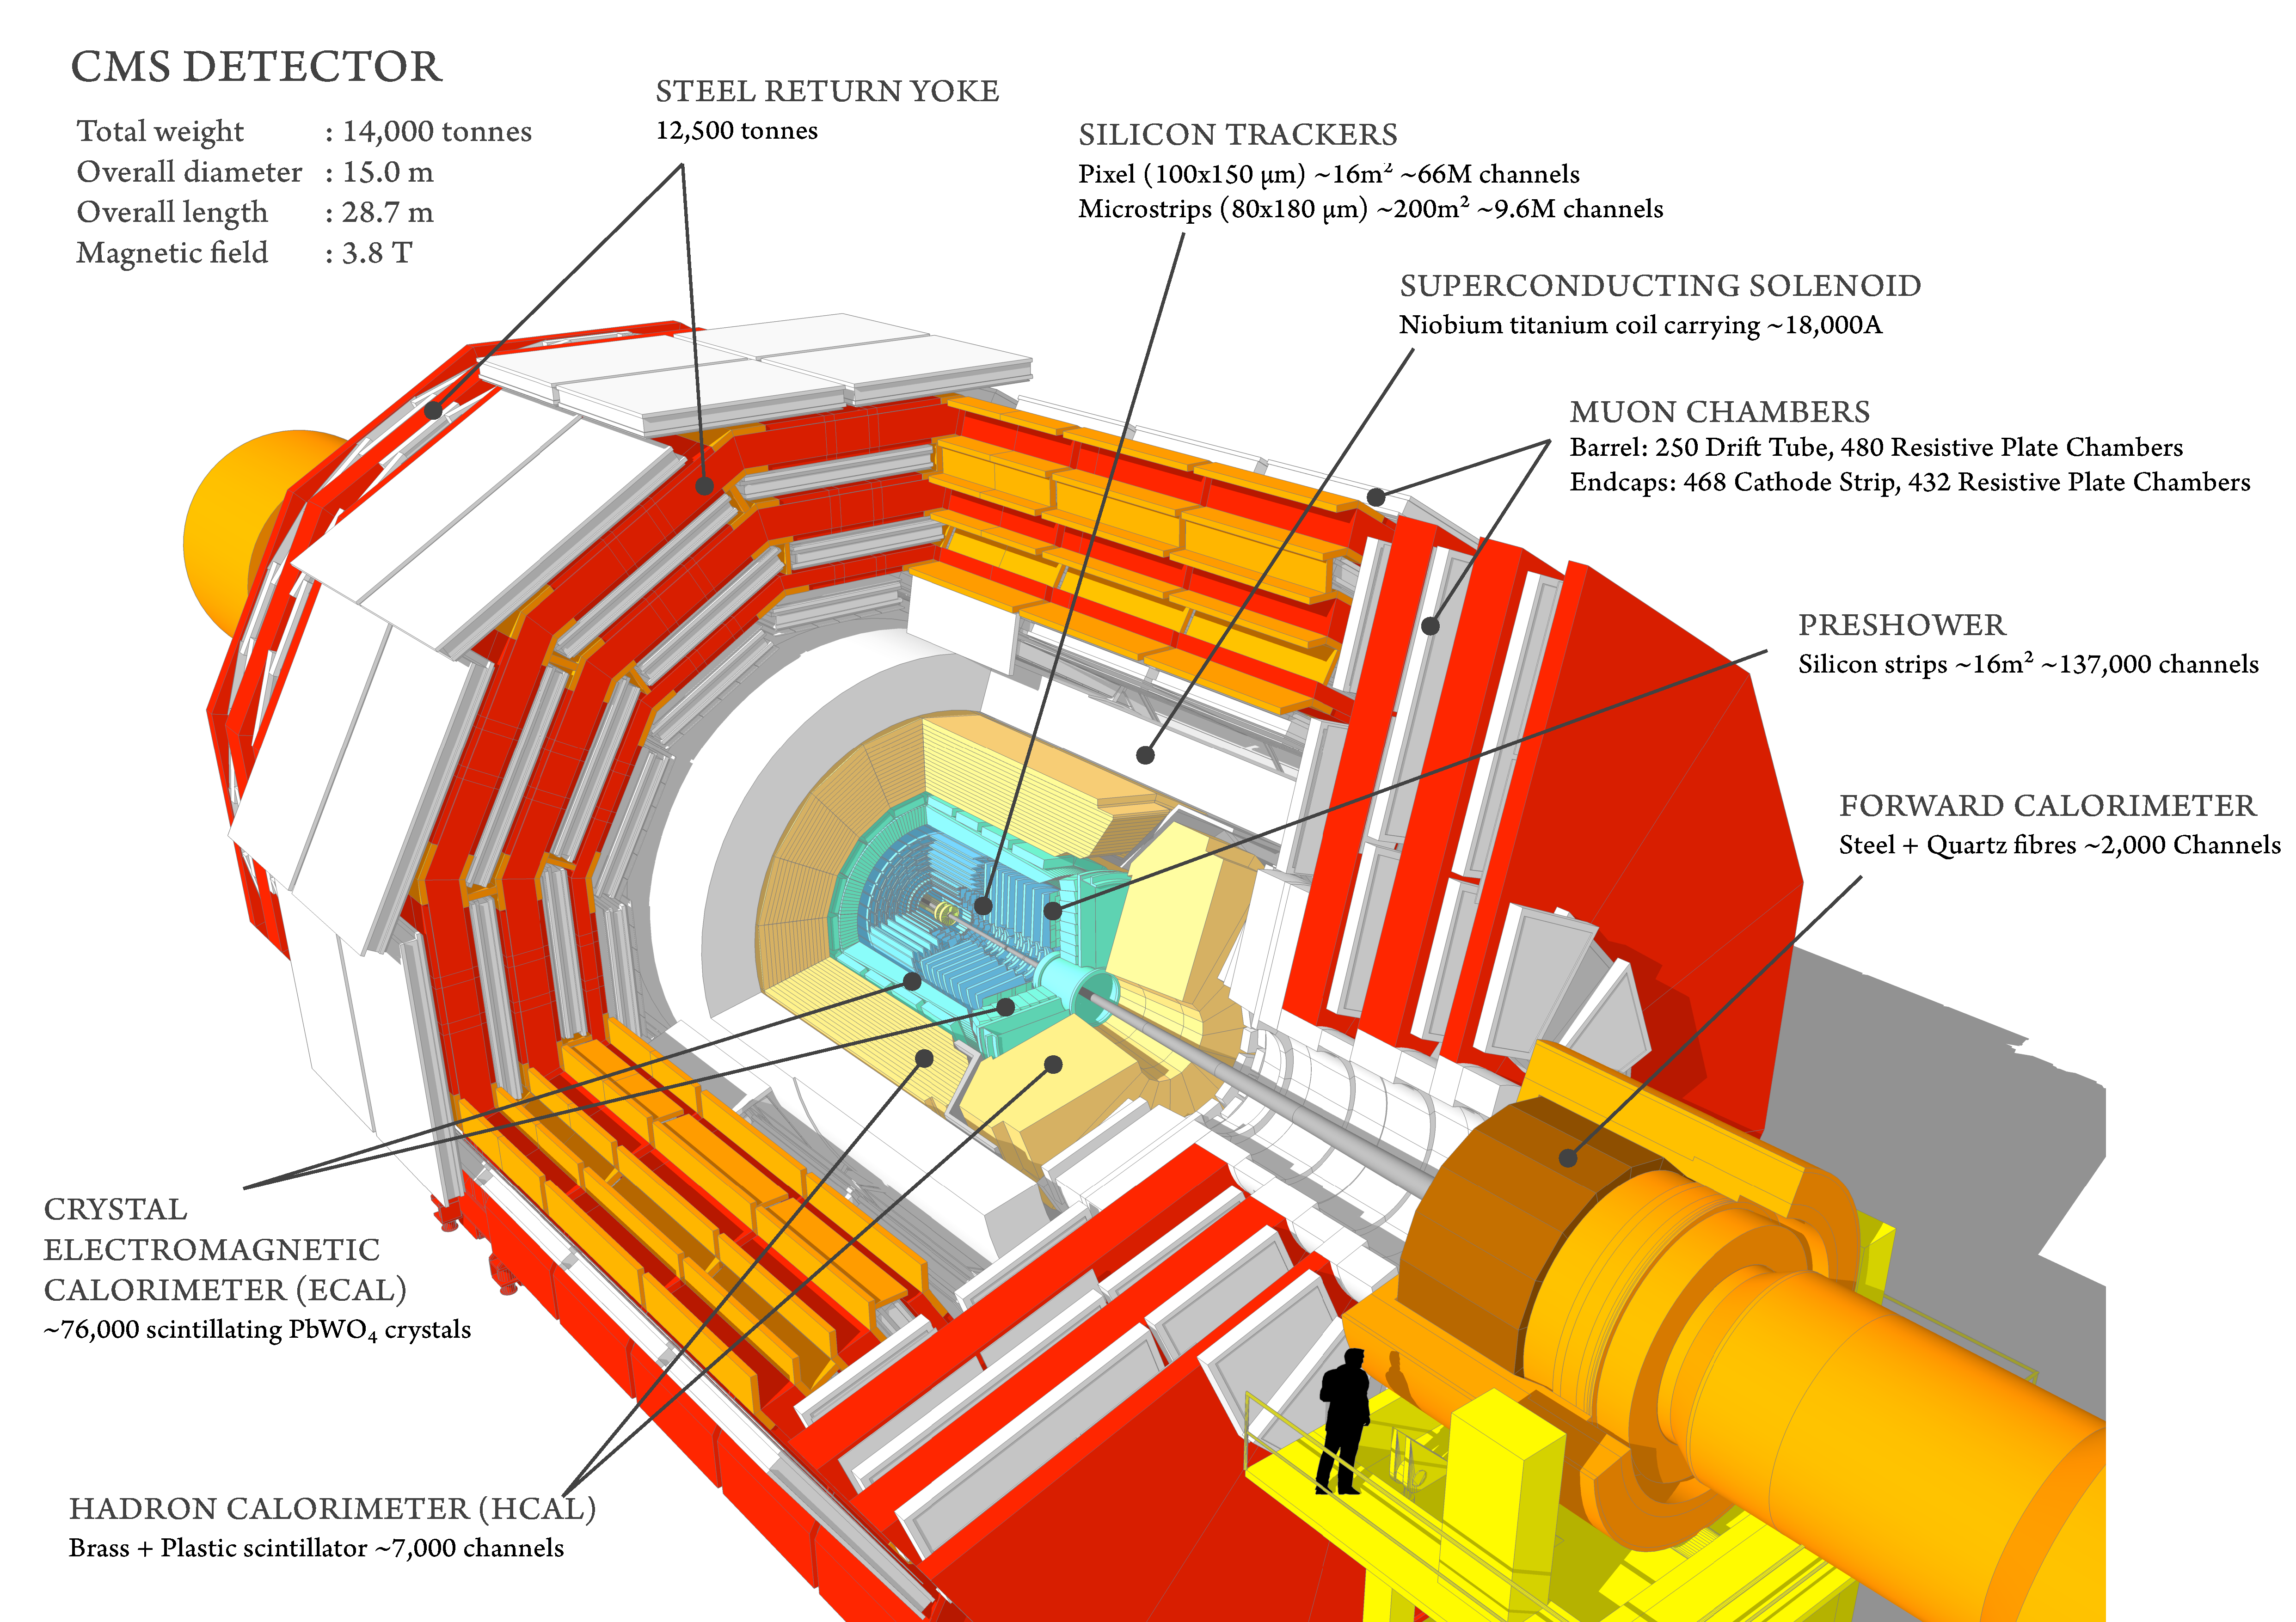
\includegraphics[width=\textwidth]{figures/cms_cutaway.pdf}
    \caption{
        A cut-away view of the CMS experiment.
    }
    \label{fig:cms_cutaway}
\end{figure}

The Compact Muon Solenoid (CMS) is one of two general-purpose particle
detectors built on the LHC ring \cite{cms_tdr_1}\cite{cms_tdr_2}. CMS is
designed to detect the very high energy, sub-atomic particles that are produced
in the LHC's proton-proton collisions. CMS is designed to have a high
acceptance and efficiency for these collisions. Here acceptance indicates the
area in both physical space as well as the area in energy and momentum space in
which the detector can detect particles. Efficiency is the probability that a
particle in CMS's acceptance region is properly measured. In order to have a
high acceptance and efficiency, CMS must be both large---to cover a large area
of physical space---and dense---to cover a large area in momentum and energy
space. CMS is 21.6\meters in length, 14.6\meters in diameter, and weighs
14\kilotonne.

CMS is built as a series of nested, finite cylinders, where each cylinder is a
separate subdetector. The beams enter the detector along the axis of the
cylinder. The collision point is in the center. There are a pair of endcaps on
either side of the cylinder to increase the acceptance of the detector. The
endcaps and central region of the cylinder (call the barrel) overlap to prevent
particles from escaping undetected through the crack. A cutaway of the detector
is shown in \FIG~\ref{fig:cms_cutaway}.

The coordinate system used by CMS is as follows: the origin is the nominal
interaction point at the center of CMS, the \xaxis is defined to point to the
center of the LHC ring, the \yaxis is defined as vertically up, and the \zaxis
points counter-clockwise and tangent to the LHC ring such that it forms a
right-handed coordinate system with the \xaxis and \yaxis. CMS uses a
cylindrical coordinate system with coordinates ($\eta$, $\phi$). The azimuthal
angel $\phi$ is in the \xyplane measured from the \xaxis so that $\phi=\pi/2$
at that \xaxis, while $\eta$ is the pseudorapidity defined by

\begin{equation}
    \eta = -\logn \tan \frac{\theta}{2}
\end{equation}

where $\theta$ is the polar angle with respects to the \zaxis. The magnetic
field points along the \zaxis.

\subsection{Inner Tracking System}

The inner tracking system, referred to as the tracker, is the subdetector
closest to the interaction point. The tracker's primary purpose is to measure
the charge of particles, the momentum of these same particles, and the location
of interaction vertices---both the primary vertex, the various additional
proton-proton vertices from pileup, and the vertices of long-lived particles
like b mesons. The tracker consists two types of silicon detectors: silicon
pixels and silicon strips. The tracker covers a pseudorapidity range of $|\eta|
< 2.4$. The pseudorapidity coverage of the tracker is the determining factor
behind the $|\eta|$ bounds used in our acceptance definition, discussed in
\SEC~\ref{sec:acceptance}.

\subsubsection{Pixel Tracker}

\begin{figure}[!htbp]
    \centering
    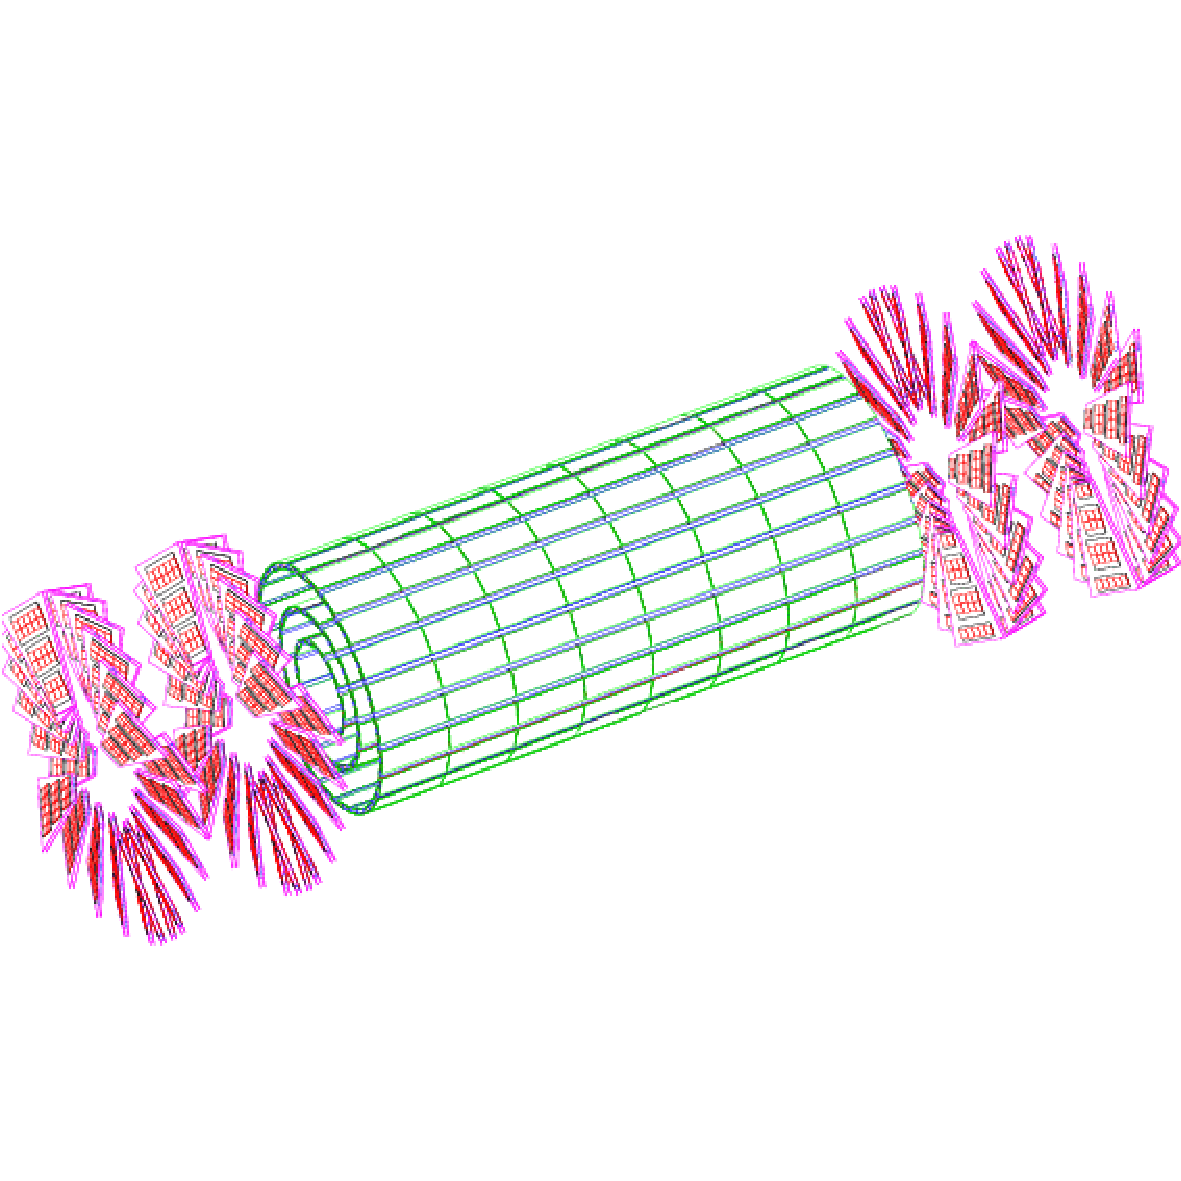
\includegraphics[width=\textwidth]{figures/pixel_layout.pdf}
    \caption{
        A rendering of the CMS pixel Tracker.
    }
    \label{fig:pixel_layout}
\end{figure}

The silicon pixels are used in the region closest to the beam pipe where the
particle flux is the highest and hence the finest granularity is needed. Their
primary purpose is to very accurately locate the primary and secondary vertices
in a collision.

There are three barrel layers of the pixel tracker at radii of of 4.3, 7.3, and
10.2\centimeters, each with a length of 53\centimeters. At each end, there are
two endcap annular disks as well placed at $|\coordz|=$ 34.5 and
46.5\centimeters. Each of these disks has an inner radius of 6\centimeters and
an outer radius of 15\centimeters.

Each pixel has an area of $100 \times 150 \micrometers^{2}$, but the resolution
of the tracker is better than that because of charge sharing. If a charged
particle ionizes multiple pixels, then a weighted average of the charges can be
used to get sub-pixel resolution on the location of the hit. In order to
increase the charge sharing, a large Lorentz angle (23\degrees) is used. The
blades which make up the endcap disks are fanned out in a turbine-like geometry
with a rotation of 20\degrees to benefit from the same effect. The layout of
the pixel detector is shown in \FIG~\ref{fig:pixel_layout}.

\subsubsection{Strip Tracker}

\begin{figure}[!htbp]
    \centering
    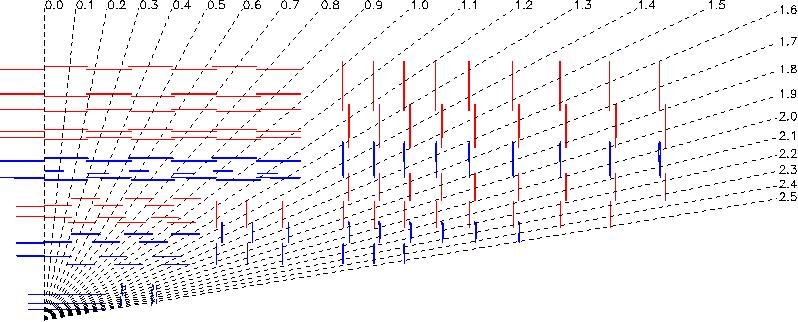
\includegraphics[width=\textwidth]{figures/strip_layout.jpg}
    \caption{
        A quarter cross section view of the CMS tracker.
    }
    \label{fig:strip_layout}
\end{figure}

The silicon strips are used further from the beam pipe than the pixels and
cover a much large radius from the beam pipe. The strip tracker has 200 times
the area of the pixel tracker, and so it was not economically feasible to use
the more expensive pixel detectors in this region. The strips' primary purpose
is to measure the momentum and curvature of the charged particles by extending
the tracker's coverage over a larger radius.

Although the strips provide only two points in space to locate a hit (as
compared to three for the pixels), this coarser geometry is adequate because of
the much lower particle flux in this region of the detector. For the momentum,
the location of the hit in the \rphiplane is the most important information,
and so the strips are aligned parallel to the magnetic field.

The strip tracker is itself divided into multiple components. In the barrel
there is the TIB (Tracker Inner Barrel) and the TOB (Tracker Outer Barrel). The
TIB consists of four layers and has coverage up to $|\coordz|<$ 65\centimeters.
The silicon sensors making up the TIB have a strip pitch which varies between
80 to 120\micrometers and have a thickness of 320\micrometers. The first two
layers are constructed with a double layer of modules with a stereo angle of
100\millirads, providing information about the location of the hit in both the
\coordrphi and \rzplane. The TOB consists of six layers and has coverage up to
$|\coordz|<$ 110\centimeters. The TOB has a strip pitch which varies between
120 and 180\micrometers and have a thickness of 500\micrometers. The thicker
sensors are able to be used in this region because the radiation levels are
lower. Having a thicker sensors helps to maintain a high signal-to-noise ratio.
Just like the TIB, the first two layers of the TOB are also built with a double
layer of modules with a stereo angle of 100\millirads.

The ends of the strip tracker consists of the TEC (Tracker Endcap) and the TID
(Tracker Inner Disk). The TEC consists of nine disks in the region
120\centimeters $< |\coordz| <$ 280\centimeters. The TID consists of three
disks in between the end of the TIB and the start of the TEC. The TEC and TID
consist of modules arrayed in rings around the beam line, with the face of each
module pointed towards the interaction point so that they have varying
orientations depending on their distance from the interaction point. The first
two rings of the TID and the first, second, and fifth rings of the TEC are
built with double layer of modules. The modules in the TID and the first three
disks of the TEC have a thickness of 320\micrometers while the rest of the
modules in the TEC have a thickness of 500\micrometers. The strip pitch in the
TID and the first three disks of the TEC have a strip pitch which varies
between 97 and 143\micrometers while the rest of the modules in the TEC have a
strip pitch between 143 and 183\micrometers. The layout of the entire tracker,
including the strip tracker, is shown in \FIG~\ref{fig:strip_layout}.

\subsection{Electromagnetic Calorimeter}
\label{ssec:ecal}

\begin{figure}[!htbp]
    \centering
    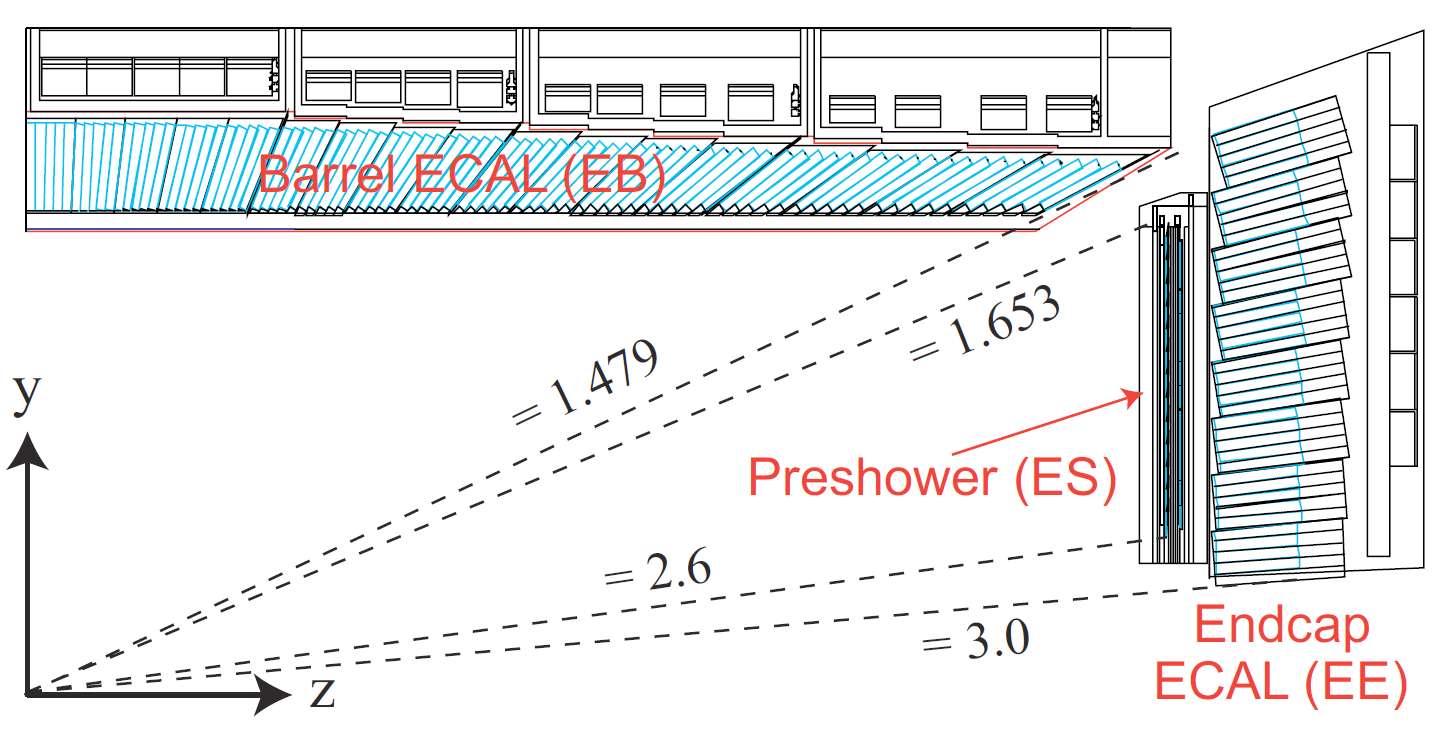
\includegraphics[width=\textwidth]{figures/ecal_layout.png}
    \caption[
        A quarter cross-sectional view of the CMS Electromagnetic calorimeter.
    ]{
        A quarter cross-sectional view of the CMS Electromagnetic calorimeter
        showing the barrel (EB), endcap (EE), and preshower (ES) components.
    }
    \label{fig:ecal_layout}
\end{figure}

The electromagnetic calorimeter (ECAL) in CMS is built around the tracker. Its
primary purpose is to measure the energy of electrons and photons. ECAL's
design was motivated by the need to measure the \higgstogammagamma decay. In
order to have suitable energy resolution, most of the energy of the particle
must be contained within the calorimeter, and so ECAL had to be very dense. In
order to separate the highly boosted photons, ECAL needed to have fine
granularity. Due to the high luminosity of the LHC, ECAL had to be radiation
hard.

In order to meet the three design goals, ECAL is made out of 75848
scintillating lead tungstate (\leadtungstate) crystals: 61200 in the barrel,
and 7324 in each of the two endcaps. The radiation length in lead tungstate is
short ($\radlength = 0.89\centimeters$) allowing ECAL to be compact (a
necessity since it must fit within the solenoid) but still contain $\approx
25\radlength$ of scintillator. The \Moliere radius is also small
(2.2\centimeters) allowing showers to be contained within each crystal. Lead
tungstate is also radiation hard (up to 10\megarads). While lead tungstate has
a fast response (80\% of light is given off within 25\ns), it does not produce
very much light ($30 \photon / \MeV$) and so sensitive photodetectors that can
operate within a strong magnetic field are required. In the barrel avalanche
photodiodes are used, and in the endcaps vacuum phototriodes are used.

\subsubsection{Electromagnetic Calorimeter Barrel}

The ECAL barrel detector (EB) has an inner radius of 129\centimeters and covers
a pseudorapidity range from $0 < |\eta| < 1.479$. It is composed of 36
identical ``supermodules'' each covering half the barrel's length and 1/18th of
the barrel's circumference. The crystals used in the EB have a front face
cross section of $22 \times 22\millimeters^{2}$ and a length of
230\millimeters. They cover 1\degrees in $\Delta \eta$ and $\Delta \phi$. The
crystals are tilted with their axis 3\degrees off from the vertex region in
order to obscure the small gaps between crystals from particles leaving the
interaction point.

\subsubsection{Electromagnetic Calorimeter Endcap}

The ECAL endcap detectors (EE) are located with their front face at
$|z|=314\centimeters$ and cover a pseudorapidity range of $1.479 < |\eta| <
3.0$. Each endcap is composed of two ``Dees'' consisting of semi-circular
aluminum plates with crystals mounted on them. The crystals used in the EE have
a front face cross section of $28.6 \times 28.6\millimeters^{2}$ and a length
of 220\millimeters. Unlike in EB, where the crystals are arranged in an
\coordetaphi~grid, the crystals in EE are arranged in an \coordxy~grid. Like
the EB crystals, the EE crystals also off-point from the vertex region.

\subsubsection{Electromagnetic Calorimeter Preshower}

In addition to EB and EE, there is a smaller subdetector, the preshower (ES),
placed in front of EE. It is made of lead and silicon and has higher
granularity then EE. It was designed to help differentiate \pitogammagamma
decays from \higgstogammagamma decays.

The layout of ECAL is shown in \FIG~\ref{fig:ecal_layout}.

\subsection{Hadronic Calorimeter}
\label{ssec:hcal}

\begin{figure}[!htbp]
    \centering
    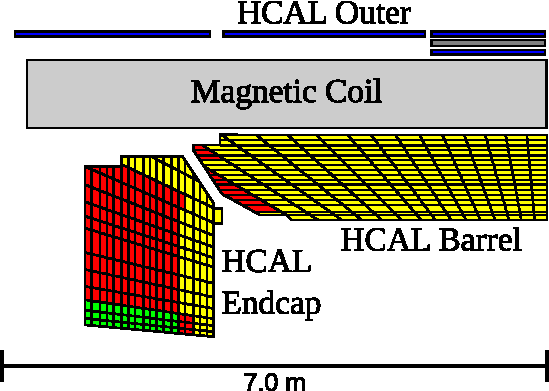
\includegraphics[width=\textwidth]{figures/hcal_cross_section.pdf}
    \caption[
        A quarter cross-sectional view of the CMS hadronic calorimeter.
    ]{
        A quarter cross-sectional view of the CMS hadronic calorimeter showing
        the barrel (HB), endcap (HE), and outer (HO) components. Not shown is
        the forward calorimeter (HF).
    }
    \label{fig:hcal_layout}
\end{figure}

The hadron calorimeter (HCAL) in CMS is built around ECAL and inside the
solenoid. HCAL's primary purpose is to measure the energy of the various
strongly-interacting particles created by the collision. HCAL must have good
containment of hadronic particles so that the missing transverse energy, \MET,
of an event can be accurately measured. This variable is useful for identifying
non-interacting particles like neutrinos, dark matter, or other long-lived
exotic particles.

HCAL is a sampling calorimeter which is appealing because that allowed it to be
made compact (and HCAL must fit within the magnet), cheap (ECAL was expensive,
so savings elsewhere were necessary), and with good enough resolution, since
the resolution is dominated by the hadronic over electromagnetic (\HOverE)
correction anyway. This correction arises from the fact that the detector
response from electromagnetic interactions is different than for hadronic
interactions, and from the fact that there are statistical fluctuations in the
number of neutral pions---which decay to two photons and so interact
electromagnetically---and charged pions---which interact hadronically---which
make up a hadronic shower in HCAL on an event-by-event basis. These differences
are corrected for in aggregate, with the effect of broadening the calorimeter's
resolution.

\subsubsection{Hadron Barrel, Hadron Endcaps, and Hadron Outer}

The hadron barrel (HB) and hadron endcaps (HE) detectors are constructed of
alternating layers of absorber and scintillators. The absorber is made of brass
because it has a short interaction length, is easy to machine, and is
nonmagnetic. In between, the showers are sampled by plastic scintillator tiles
read out with embedded wavelength-shifting fibers. The wavelength-shifting
fibers are spliced to clear fibers outside the scintillator which carry the
signal to the readout system. The light is readout by multi-channel hybrid
photodiodes. The hadron outer (HO) detector is a layer of plastic scintillator
on the outside of the solenoid before the muon systems begin. It serves as a
``tail catcher'' by measuring the hadronic energy leaking through HCAL and
interacting with the magnet.

%HB consists of 72 segments of 32 towers with each segment covering a
%pseudorapidity range from $0 < |\eta| < 1.4$. The size of each tower is $\Delta
%\eta \times \Delta \phi = 0.087 \times 0.087$. In HB there are 15 brass plates,
%each with a thickness of 5\centimeters and two stainless steel plates, one on
%the inner face and one on the outer face to add mechanical strength. The first
%scintillator plate has a thickness of 9\millimeters, all others have a
%thickness of 3.7\millimeters. HE, unlike EE, is constructed to form a grid in
%\coordetaphi. It covers a rapidity region from $1.3 < |\eta| < 3$. For the
%lowest values of $\eta$ its channel size roughly matches the barrel, but this
%size grows at higher $\eta$.

\subsubsection{Hadron Forward}

The hadron forward (HF) calorimeter is the most forward of of the detectors
that make up HCAL, and the one of the most forward detectors in CMS. HF is
located 11.2\meters from the interaction point. It covers a pseudorapidity
range of $3 < |\eta| < 5$ and so receives a very high particle flux. HF must be
very radiation hard in order to survive in this environment. HF is constructed
of steel and quartz. The signal in HF originates from \Cherenkov light in the
quartz.

The steel absorb is 1.65\meters thick. Placed within the absorber are quartz
fibers which are 0.6\millimeters in diameter and oriented parallel to the
\zaxis. These fibers are arranged in a square grid 5\millimeters apart. There
are two lengths of fibers: ``long'' 1.65\meters ones and ``short'' 1.43\meters
ones. These different lengths allow HF to sample showers at two different
depths.

The layout of HCAL is shown in \FIG~\ref{fig:hcal_layout}.

\subsection{Magnet}

The central feature of CMS, both from a design standpoint and structurally, is
the large superconducting solenoid magnet. A high strength magnetic field is
required in CMS in order to achieve a momentum resolution of $\Delta \momentum
/ \momentum \approx 10\%$ for muons with $\momentum = 1 \TeV$. The momentum of
these muons must be measured using their curvature in the tracker and the muon
chambers. Additionally, the magnetic field allows the charge of particles to be
measured by the direction in which their tracks curve. The solenoid provides a
magnetic field for all of the components inside the bore of the magnet. The
fringing fields are collected and returned by the iron return yokes which also
support the muon chambers. In this way a field is provided for the muon
chambers without requiring an additional magnet.

The solenoid is 12.9\meters long with an inner bore of 5.9\meters. It generates
a 3.8\tesla field using 2168 turns of conductor which carry 19.5\kiloamps. The
total stored energy is 2.7\gigajoules. The solenoid is encased in aluminum to
help dissipate heat and add strength. This entire assembly is enclosed in a
stainless steel cryostat. The cryostat must be exceptionally strong because it
not only supports the solenoid, but also all of the barrel subdetectors (HCAL,
ECAL, and the tracker) that are mounted within it. The calorimeters and the
tracker are mounted within the solenoid in order minimize the un-instrumented
mass---where particles could lose energy due to interactions---between the
calorimeters and the collision region.

\subsection{Muon System}

\begin{figure}[!htbp]
    \centering
    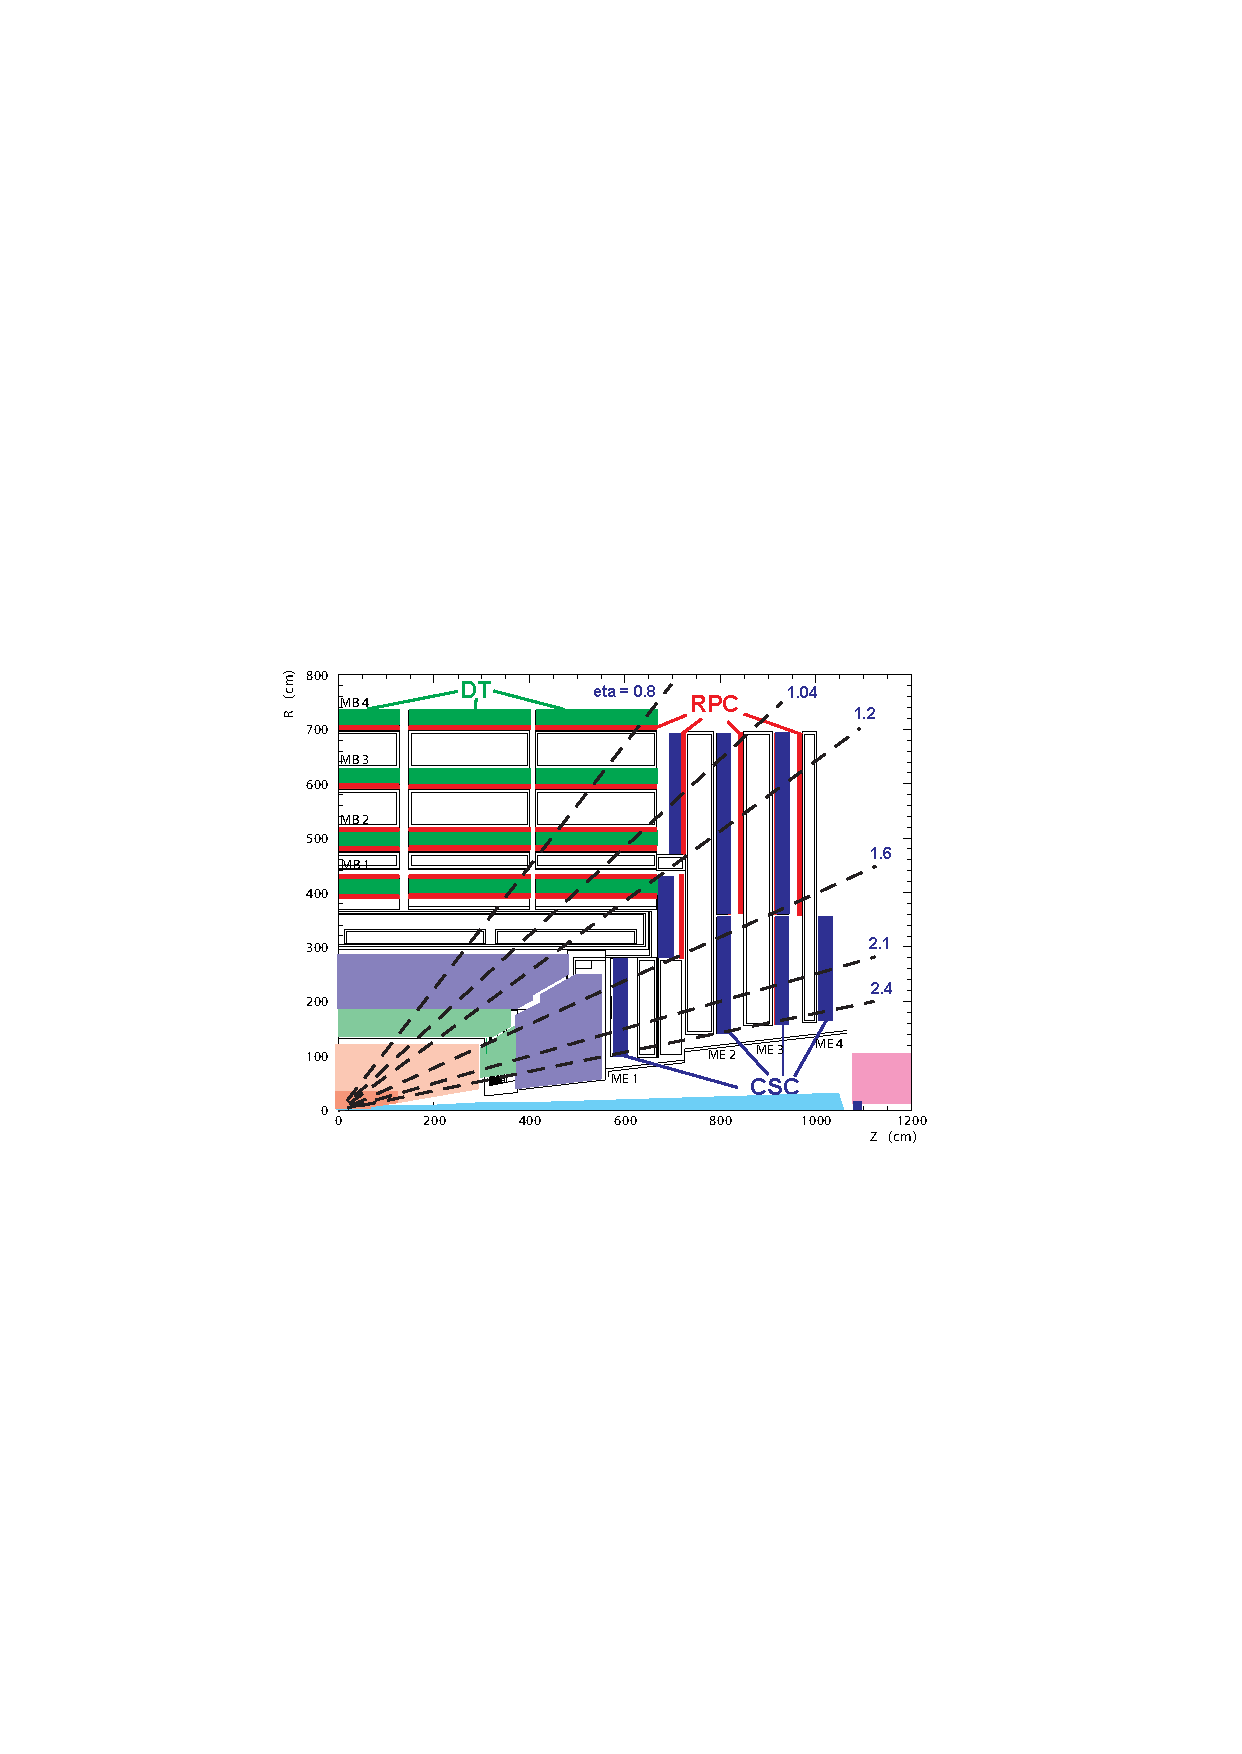
\includegraphics[width=\textwidth]{figures/muon_layout.pdf}
    \caption[
        A quarter cross-sectional view of the CMS muon system.
    ]{
        A quarter cross-sectional view of the CMS muon system showing the drift
        tubes (DT), cathode stripe chambers (CSC), and resistive plate chambers
        (RPC).
    }
    \label{fig:muon_layout}
\end{figure}

The muon system is the outer most subdetector of CMS. Its primary purpose is to
assist in measuring high momentum muons and to allow triggering on muons.
Without the muon system, no triggering on muons would be possible because they
are minimum ionizing particles in the calorimeters and the tracker can not be
read out quickly enough to use in triggering. For high energy muons ($\pt > 200
\GeV$), a combination of the tracker and muon system provides the most accurate
measurement because of the increased lever arm provided by the muon system. The
muon chambers are built within the iron return yokes and as such are outside
the primary magnetic field provided inside the solenoid.

The muon systems must cover a very large surface area, $25,000\meters^{2}$, and
so gaseous detectors are used in order to keep the cost down. Three types of
gaseous detectors are used in the muon system: drift tube (DT) chambers,
resistive plate chambers (RPC), and cathode strip chambers (CSC),

\subsubsection{Drift Tubes}

DTs are gas ionization detectors with an anode wire strung down the center of
each tube which act as the cathode. The wire collects the ionization charged
caused by a muon passing through the tube. By using a timing and pulse shape
measurement, the DTs can achieve a point resolution of $\approx
200\micrometers$ leading to a position resolution in $\phi$ of 100\micrometers
and a direction measurement good to approximately 1\millirads. The maximum
drift length in the DTs is 2\centimeters.

\subsubsection{Resistive Plate Chambers}

The RPCs are constructed of two parallel high-voltage plates. When a muon
passes through it causes an electron cascade that is collected on the anode,
which is divided into strips to allow the position of the cascade to be
measured. RPCs have worse position resolution than the DTs, but are much
faster because they have a shorter drift length, with a timing response of
$\approx 1\ns$.

\subsubsection{Cathode Strip Chambers}

The CSCs are flat gas chambers with parallel anode wires running the length on
one side, and cathode wires on the other side running orthogonal to the anodes.
A prompt signal is provided by the anode wires, while a weighted average of the
image charge on the cathode provides a slower but more precise location. The
anode signal is used in triggering at \Lone while the cathodes are used for
final reconstruction. The spatial resolution of $\approx 200\micrometers$
($100\micrometers$ in the first ring of the first endcap disk) and the angular
resolution in $\phi$ is $\approx 2\millirads$.

\subsubsection{Muon System Barrel}

In the barrel region ($|\eta| < 1.2$) DTs are used because the induced neutron
background is low, the muon rate is low, and the magnetic field is low. RPCs
are also used in the barrel to augment the DTs. The barrel consists of four
layers of muon stations in five wheels corresponding to the five wheels making
up the iron return yoke. Each wheel has 12 sectors that cover 30\degrees. The
chambers are staggered such that a high energy muon produced near the boundary
must cross 3 of the 4 layers. Of the three inner layers has 12 chambers, and
the 4th layer has 2 chambers in the bottom and top sectors, and so has 14
chambers in total. The first three layers are aligned to measure in \coordrphi
and \coordz, while the 4th layer measures only in \coordrphi. Each chamber
consists of 12 planes of DTs with 2 RPCs---1 on the front and 1 on the
back---in the first two layers, and 1 RPC---on the front---for the second two
layers.

\subsubsection{Muon System Endcap}

In the endcap region the higher magnetic field, neutron background, and muon
flux make DTs ineffective and so CSCs are used instead. There are three disks
of CSCs chambers with RPCs sandwiched between disks of the iron return yoke in
the rapidity range $|\eta| < 1.6$. After that range there are only CSCs
chambers. There are 6 CSCs per chamber.

The layout of the muon system is shown in \FIG~\ref{fig:muon_layout}.

\subsection{The Trigger}
\label{ssec:trigger}

The trigger's job is to select the interesting physics events from all of the
collisions happening in CMS. The trigger must be able to handle the full bunch
crossing rate at the LHC of 40\megahertz (although it only ran at 20\megahertz
in 2012). The trigger accomplishes this by using a two level design. The first
level, the \Lone (L1) trigger, consists of custom hardware cuts the
20\megahertz of collisions down to about 100\kilohertz. These events are then
passed to the second level of the trigger, the high-level trigger (HLT), which
uses software running on commodity hardware to select 1\kilohertz of events.

\subsubsection{The \Lone Trigger}

The L1 trigger is implemented in custom hardware because it must be incredibly
fast. Each event is given just 3.2\microseconds to travel from the detector to
the service cavern and be accepted or rejected by the L1 trigger. Of this time,
less than 1\microseconds is given for the L1 trigger to make its decision. The
L1 trigger only uses information from the muon system and the calorimeters; it
does not use information from the tracker as it takes too long for this
data to be assembled and transfered. From the calorimeters the L1 trigger gets
the sum of energy in a fixed array of \fivebyfive crystals in ECAL as well as
the energy behind each array in HCAL. From the muon chambers the L1 trigger
gets a short vector from each detector indication the location of a hit in the
chamber and the direction the particle was traveling in. The L1 trigger also
makes use of a few global sums including \ET and \MET.

While a decision is being made, the data from the collision are stored in a
hardware buffer. If the L1 trigger selects the event, the data are moved from
the buffer and sent to the central DAQ system where it is held until all the
data are assembled, at which point it is sent to one of the computers that makes
up HLT.

\subsubsection{The High-Level Trigger}

The HLT is implemented in the same software that is used for offline analyses.
Running the same analysis software as is used offline allows HLT to access the
full range of data from every part of the detector and use any reconstruction
or selection algorithm available offline. This allows very sophisticated
triggers to be written, and additionally allows triggers to be easily modified
as conditions change. The HLT is designed so that the simplest triggers are run
first, with more sophisticated---and hence computationally expensive---triggers
running later if needed.

HLT runs on a server farm consisting of commodity hardware. There are currently
around 10,000 processor cores in the HLT farm. By using commodity server
hardware, HLT benefits from the rapid speed and power advances that are being
made in commercial computing.
